\documentclass[12pt]{article}

\usepackage[margin=1in]{geometry}
\usepackage{amsmath,amssymb}
\usepackage{graphicx}
\usepackage{booktabs}
\usepackage{float}
\usepackage{hyperref}
\usepackage{parskip}
\usepackage{array}

\title{\textbf{LiDAR-Based 3D Object Classification for Pattern Recognition Using a PointNet-Style Neural Network}}
\author{Mohamed Elgouhary}
\date{}

\begin{document}

\maketitle

\begin{abstract}
This project investigates a pattern-recognition problem based on 3D LiDAR point clouds from the KITTI object dataset. The objective is to classify cropped LiDAR object point clouds into three semantic categories: Car, Pedestrian, and Cyclist. A balanced dataset was constructed by extracting object-level point clouds from KITTI training frames, filtering sparse crops, normalizing each sample, and resampling every point cloud to a fixed size of 1024 points. A simple PointNet-style neural network was then trained to perform object classification directly on the processed point sets. The proposed approach achieved a best validation accuracy of 97.96\% and a final test accuracy of 95.37\%. The results indicate that the model learns discriminative geometric patterns from LiDAR data effectively, with the main classification difficulty arising between pedestrians and cyclists.
\end{abstract}

\section{Introduction}

Pattern recognition is concerned with identifying meaningful structure in data and assigning observations to semantic categories. Common pattern-recognition tasks include classification, detection, clustering, and segmentation. In many classical applications, the input data is represented on a regular grid, such as a 2D image. In contrast, LiDAR data is naturally represented as an unordered set of 3D points, which introduces additional challenges for representation and learning.

This project studies a 3D pattern-recognition task in the context of autonomous driving: classifying LiDAR point clouds corresponding to road objects into semantic classes. Specifically, the goal is to distinguish among Cars, Pedestrians, and Cyclists using object crops extracted from the KITTI dataset. This is a meaningful pattern-recognition problem because the model must infer class identity from geometric structure alone, without relying on image appearance.

To keep the project focused and manageable, the task is formulated as object-level classification rather than full-scene detection or point-wise semantic segmentation. This formulation allows the study to concentrate on learning discriminative patterns from point-cloud geometry while still addressing a realistic recognition problem from autonomous driving. A PointNet-style architecture was selected because it can operate directly on unordered point sets and aggregate point-wise information into a global feature representation.

\section{Dataset and Preprocessing}

The project uses the KITTI object benchmark as the data source. From the KITTI training split, three types of files were used: Velodyne LiDAR point clouds, calibration files, and object labels. Only three semantic categories were considered in this study:

\begin{itemize}
    \item Car
    \item Pedestrian
    \item Cyclist
\end{itemize}

The original object counts in KITTI are highly imbalanced, with Cars appearing much more frequently than Pedestrians and Cyclists. To avoid training bias toward the dominant class, a balanced subset was constructed. After crop extraction, filtering, and class balancing, the final dataset consisted of:

\begin{itemize}
    \item 1200 Car samples
    \item 1200 Pedestrian samples
    \item 1200 Cyclist samples
\end{itemize}

for a total of 3600 object-level point clouds.

\subsection{Object Crop Extraction}

Each KITTI frame contains a LiDAR point cloud together with object annotations and calibration parameters. Because the object labels are defined in camera coordinates while the LiDAR points are measured in Velodyne coordinates, the LiDAR data was first transformed into rectified camera coordinates using the provided calibration matrices.

For each labeled target object, the points lying inside the corresponding 3D bounding box were extracted to form one object crop. Only objects belonging to the three target classes were retained. Crops containing fewer than 30 points were discarded in order to remove extremely sparse or unreliable samples.

\subsection{Normalization and Resampling}

The number of points varies substantially from one object crop to another, depending on object size, pose, and distance from the sensor. Since the classifier requires a fixed-size input, each crop was converted to a point cloud of shape $(1024, 3)$ using the following procedure:

\begin{enumerate}
    \item Keep only the spatial coordinates $(x,y,z)$.
    \item Subtract the centroid so that the cloud is centered at the origin.
    \item Scale the cloud to approximately fit inside a unit sphere.
    \item If the cloud contains more than 1024 points, randomly sample 1024 points without replacement.
    \item If the cloud contains fewer than 1024 points, sample with replacement until 1024 points are obtained.
\end{enumerate}

This preprocessing produces a consistent representation across all samples while preserving the overall geometric structure of each object.

\subsection{Train/Validation/Test Split}

A stratified split was used so that each class remained equally represented in the training, validation, and test partitions. The final split was:

\begin{itemize}
    \item Training set: 2520 samples
    \item Validation set: 540 samples
    \item Test set: 540 samples
\end{itemize}

Each split was class-balanced.

\section{Methodology}

\subsection{Model Architecture}

A simple PointNet-style neural network was implemented for classification. The input to the network is a point cloud of size $(1024, 3)$. A shared multilayer perceptron (MLP) is applied independently to every point in the set. The resulting point-wise features are then aggregated using a max-pooling operation across all points, producing a global feature vector that represents the entire object. This global representation is finally passed through fully connected layers to predict the class label.

The architecture used in this project is summarized below:

\begin{itemize}
    \item Shared MLP: $3 \rightarrow 64 \rightarrow 128 \rightarrow 256$
    \item Symmetric aggregation: global max pooling
    \item Classification head: $256 \rightarrow 128 \rightarrow 64 \rightarrow 3$
\end{itemize}

ReLU activations were used after the hidden layers, and dropout was applied in the classification head to reduce overfitting.

\subsection{Training Configuration}

The model was trained using the following setup:

\begin{itemize}
    \item Optimizer: Adam
    \item Learning rate: $10^{-3}$
    \item Batch size: 32
    \item Number of epochs: 30
    \item Loss function: cross-entropy loss
\end{itemize}

Training was performed on a CUDA-enabled GPU. The model with the highest validation accuracy was saved and later evaluated on the held-out test set.

\section{Experiments and Results}

\subsection{Training Behavior}

The model converged quickly and achieved strong classification performance on the validation set. The best validation accuracy obtained during training was:

\[
\boxed{97.96\%}
\]

Figures~\ref{fig:loss} and~\ref{fig:acc} show the training and validation loss and accuracy across epochs. The curves indicate stable learning behavior and strong generalization performance, with no evidence of severe overfitting.

\begin{figure}[H]
    \centering
    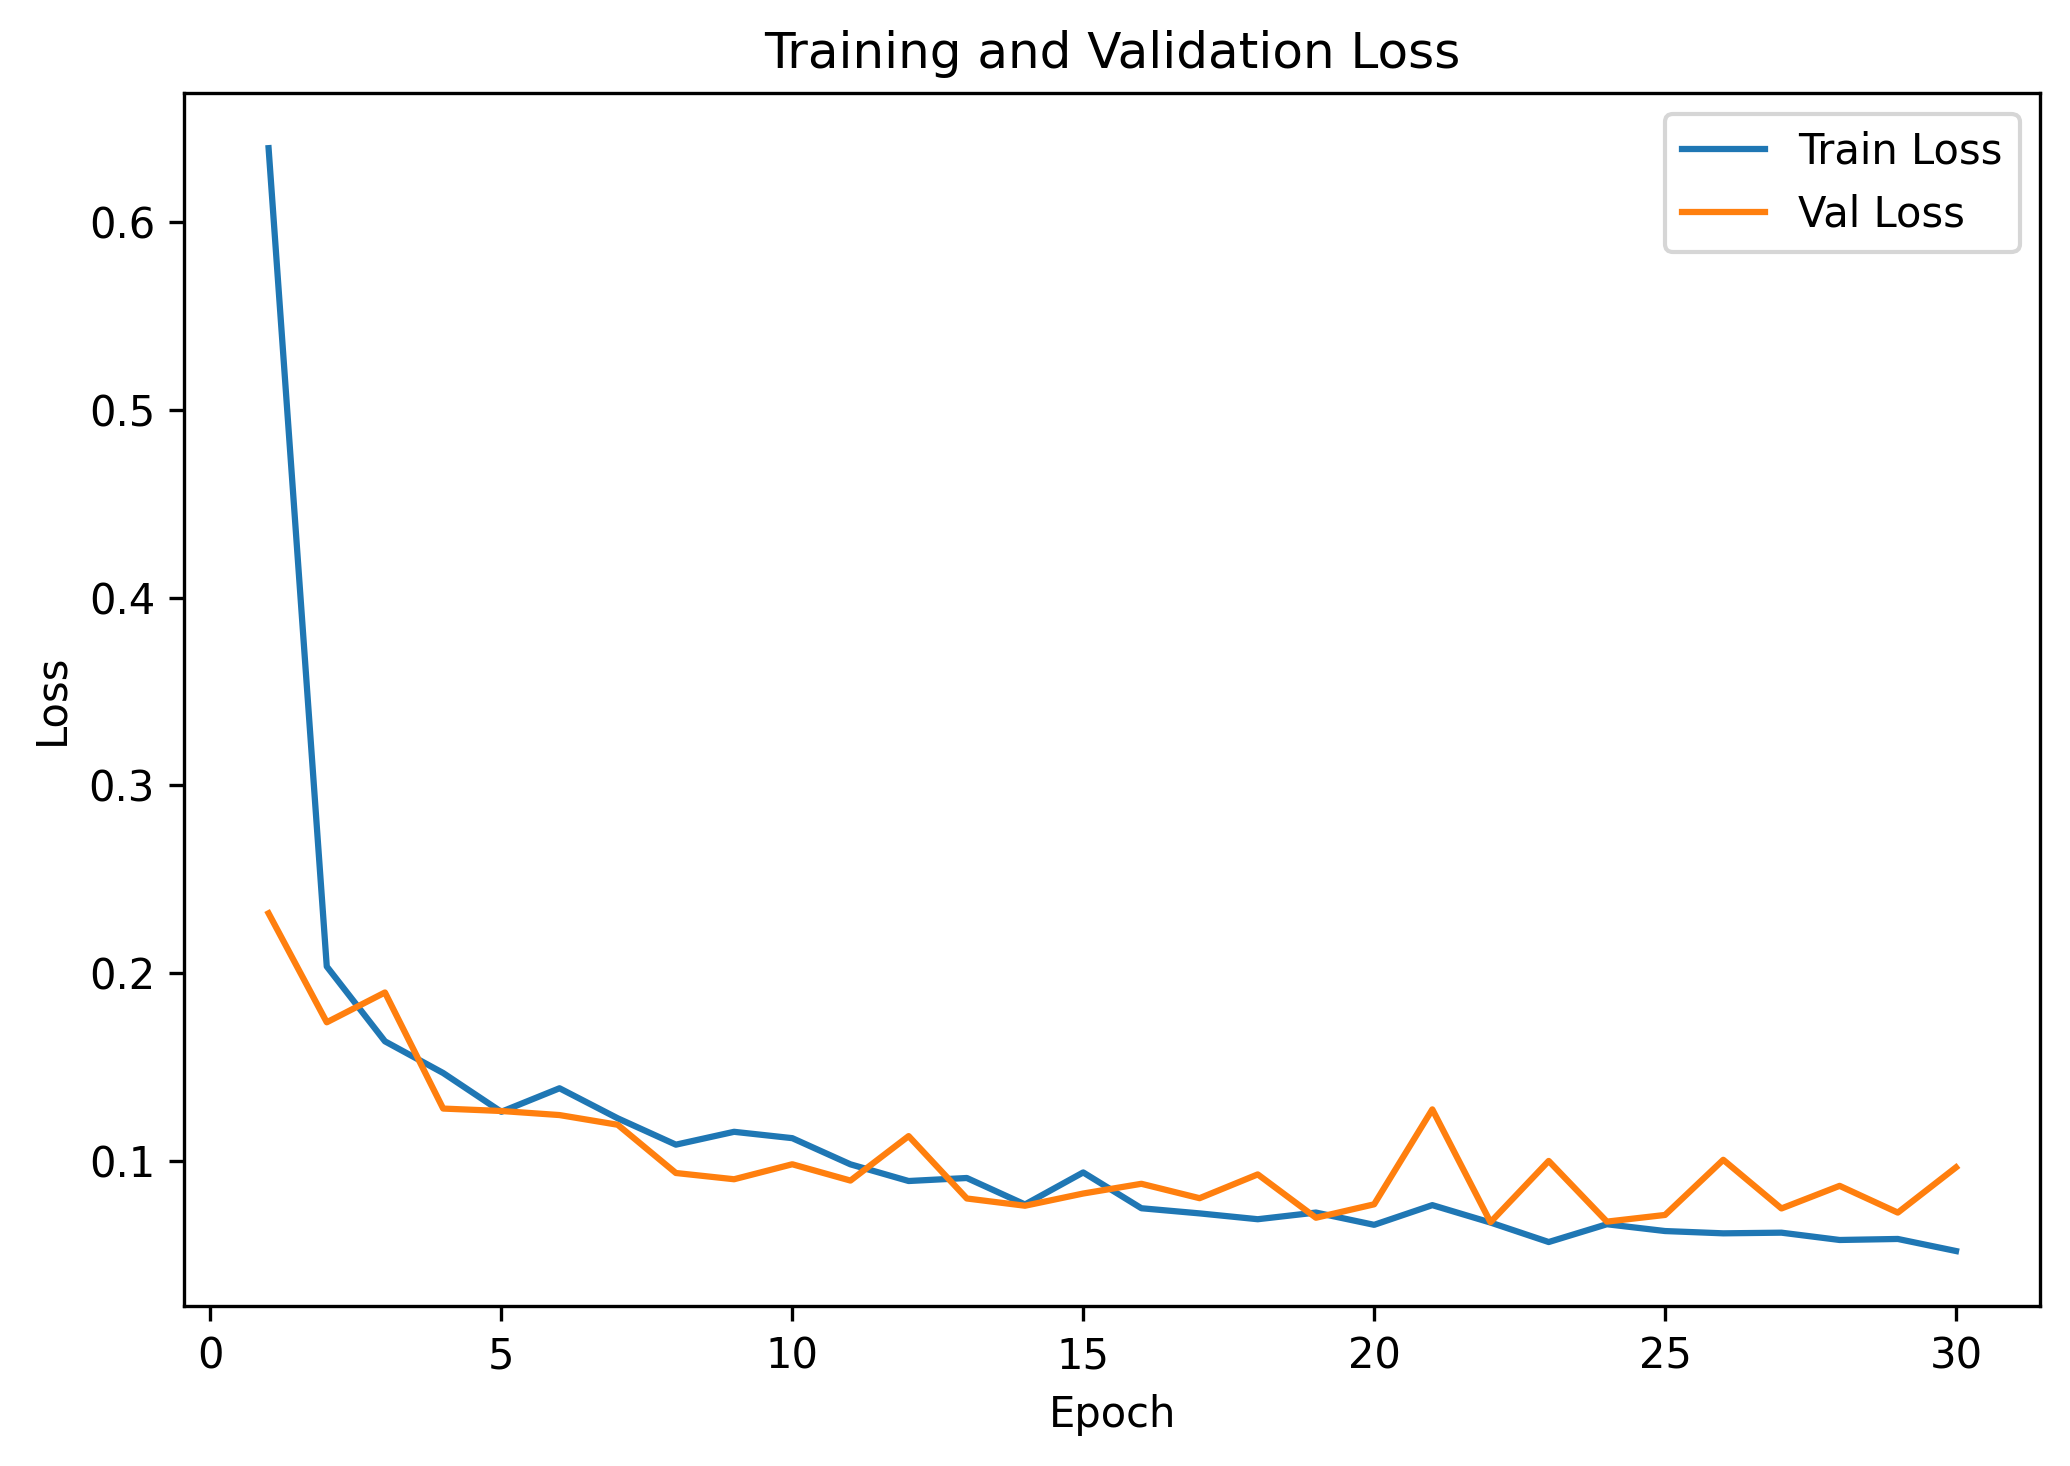
\includegraphics[width=0.75\linewidth]{loss_curve.png}
    \caption{Training and validation loss across epochs.}
    \label{fig:loss}
\end{figure}

\begin{figure}[H]
    \centering
    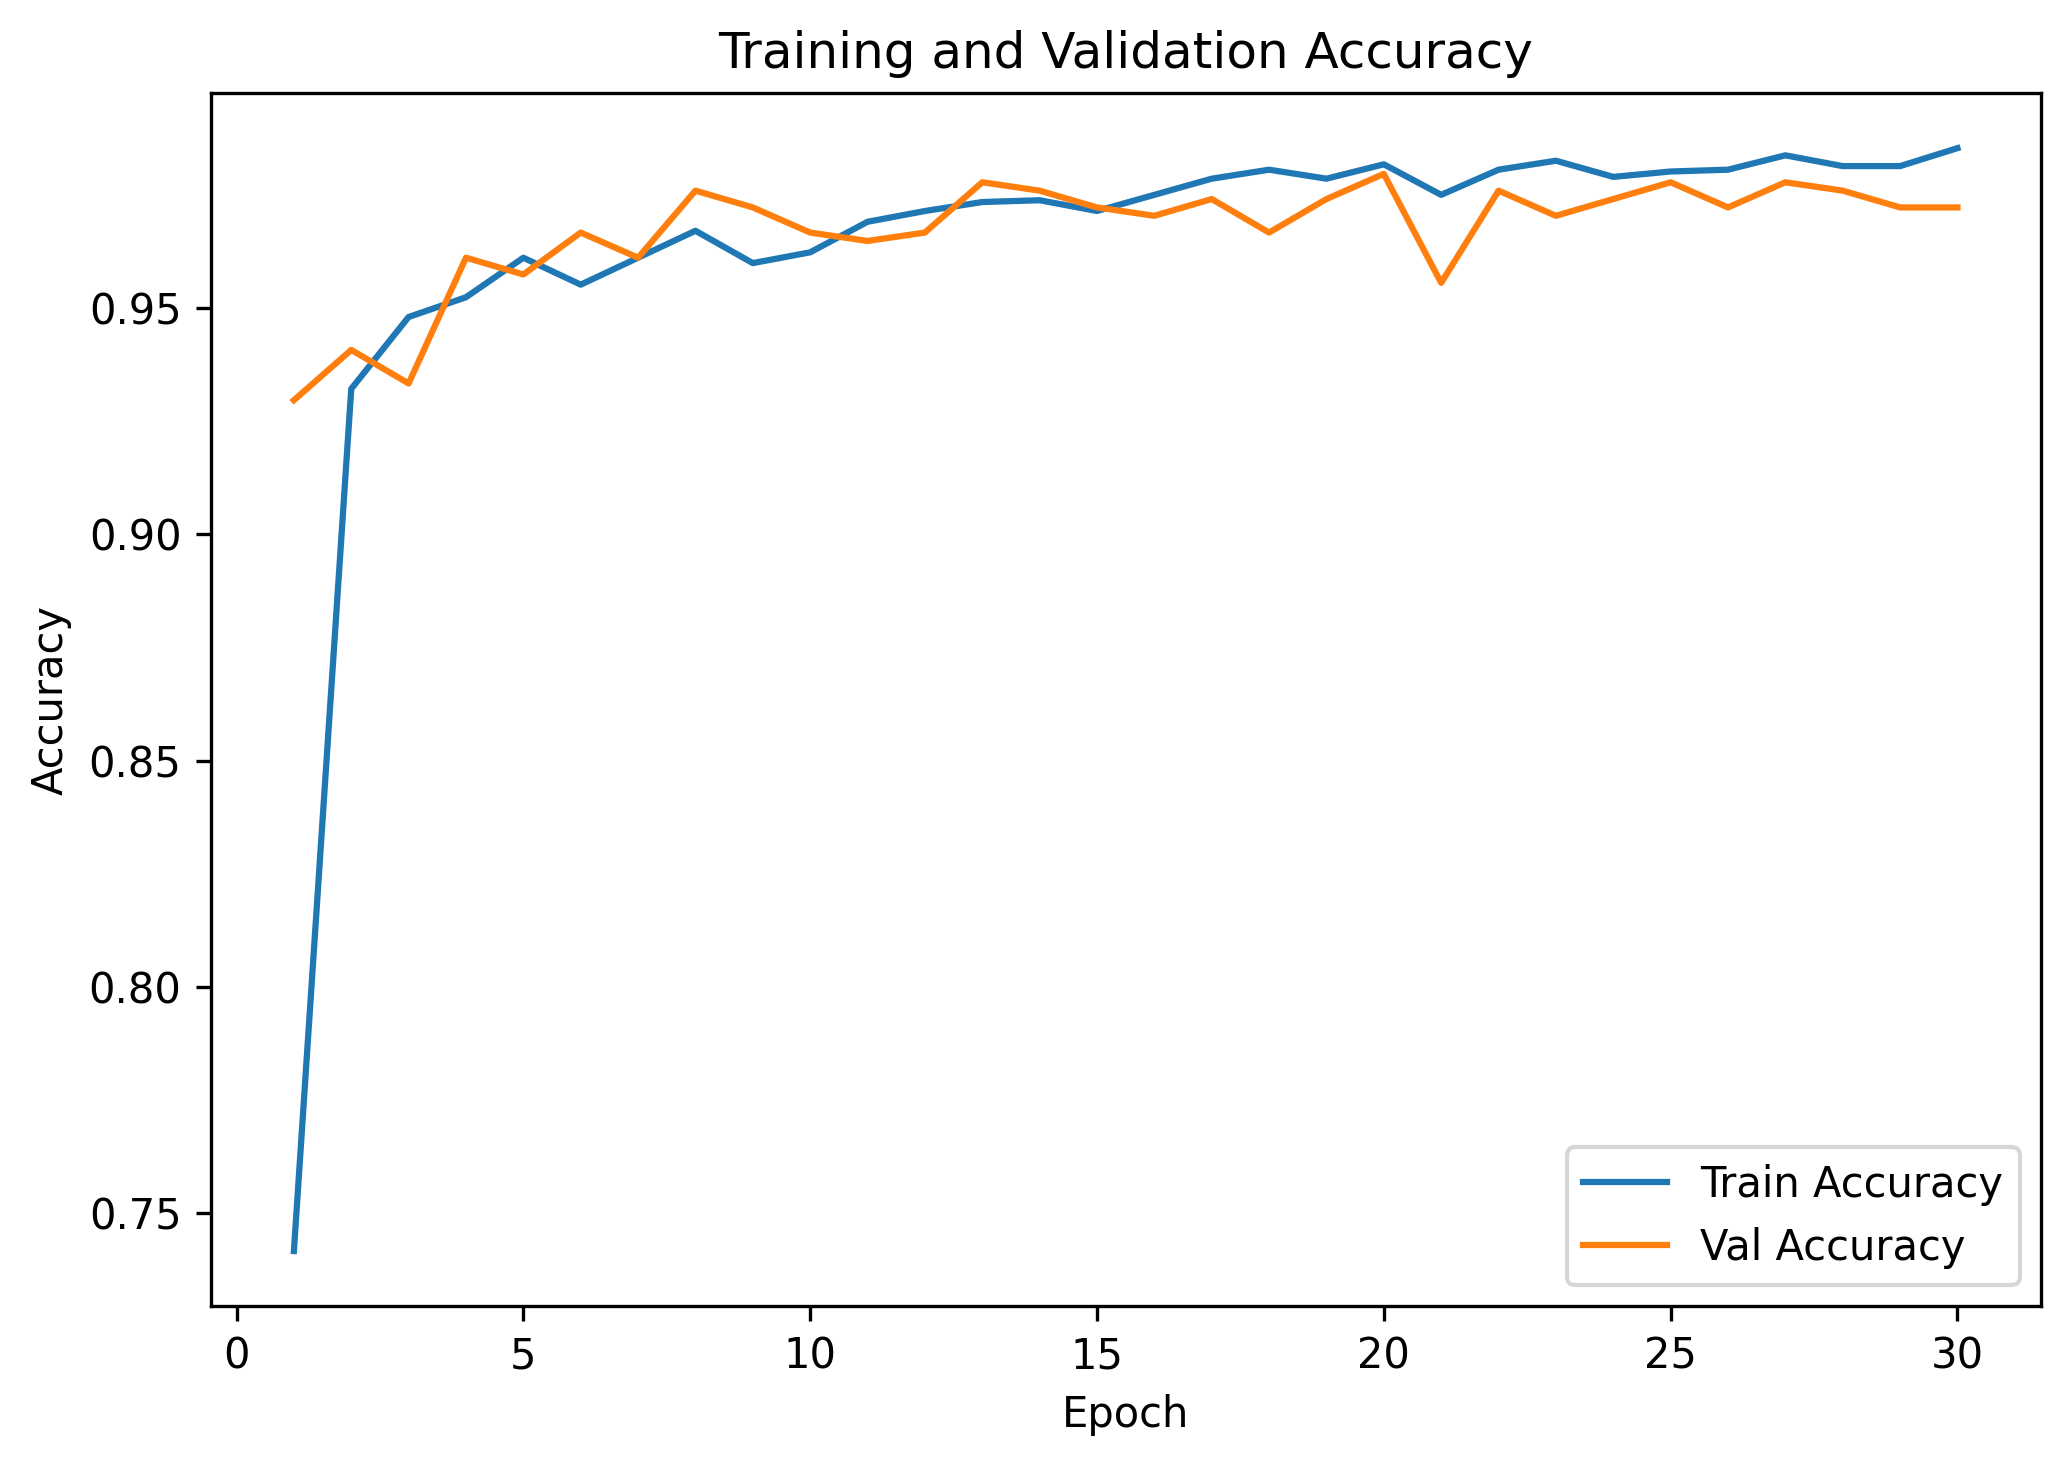
\includegraphics[width=0.75\linewidth]{accuracy_curve.png}
    \caption{Training and validation accuracy across epochs.}
    \label{fig:acc}
\end{figure}

\subsection{Test Performance}

The best saved model was evaluated on the test set. The final test accuracy was:

\[
\boxed{95.37\%}
\]

Table~\ref{tab:class_results} reports the per-class precision, recall, and F1-score.

\begin{table}[H]
\centering
\caption{Per-class classification results on the test set.}
\label{tab:class_results}
\begin{tabular}{lccc}
\toprule
Class & Precision & Recall & F1-score \\
\midrule
Car        & 0.9780 & 0.9889 & 0.9834 \\
Pedestrian & 0.9818 & 0.9000 & 0.9391 \\
Cyclist    & 0.9067 & 0.9722 & 0.9383 \\
\bottomrule
\end{tabular}
\end{table}

The confusion matrix is shown in Fig.~\ref{fig:cm}.

\begin{figure}[H]
    \centering
    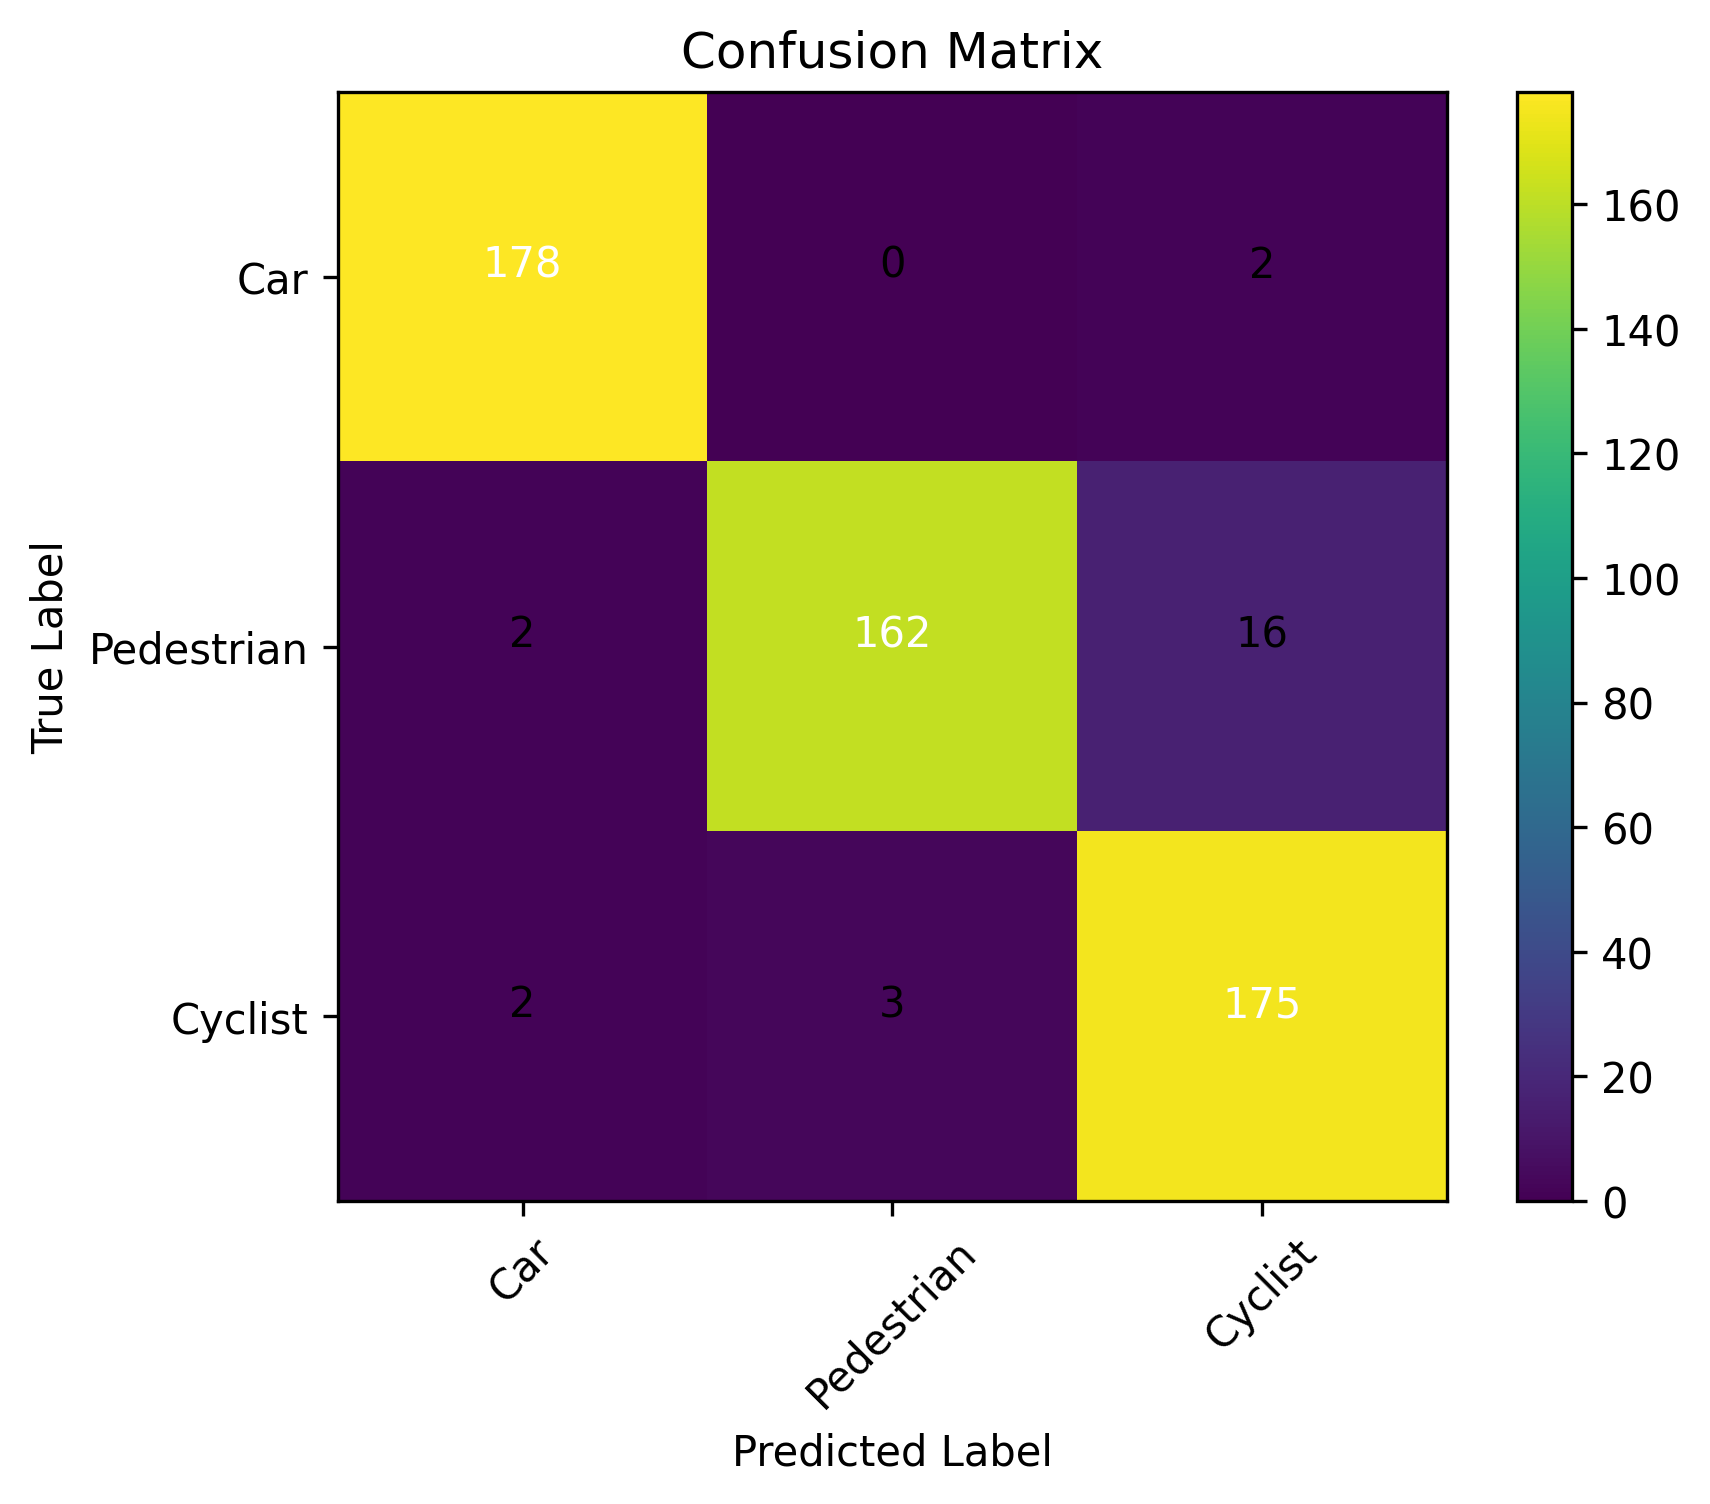
\includegraphics[width=0.65\linewidth]{confusion_matrix.png}
    \caption{Confusion matrix on the test set.}
    \label{fig:cm}
\end{figure}

\subsection{Analysis of Classification Errors}

The confusion matrix obtained on the test set is:

\[
\begin{bmatrix}
178 & 0 & 2 \\
2 & 162 & 16 \\
2 & 3 & 175
\end{bmatrix}
\]

Cars were classified most reliably, with only a few misclassifications. The most notable confusion occurred between Pedestrians and Cyclists, particularly Pedestrians being predicted as Cyclists. This behavior is understandable because these two classes can produce relatively sparse and partially similar LiDAR structures, especially when the observed object occupies only a limited number of points.

\section{Discussion}

The results demonstrate that a relatively simple PointNet-style model can achieve strong performance on LiDAR object classification. Several observations emerge from this study.

First, constructing a balanced dataset was important for preventing the Car class from dominating the learning process. Without balancing, the classifier could have achieved high overall accuracy while still performing poorly on minority classes.

Second, Cars were the easiest class to recognize. This is likely because they tend to occupy more points and exhibit more stable geometric structure than Pedestrians and Cyclists.

Third, Pedestrians and Cyclists were more difficult to separate. Both classes often appear as sparse vertical point patterns, and the difference between them may be subtle when the point cloud is limited or noisy.

Finally, the strong performance obtained with a simplified PointNet-style architecture suggests that direct learning from point sets is effective for this classification task, even without using more advanced point-cloud models.

One limitation of this project is that it focuses on object-level classification rather than full-scene detection. In addition, only three object categories were considered, and the dataset was balanced through class capping. Future work could investigate more advanced architectures such as PointNet++, graph-based point-cloud networks, or full-scene semantic segmentation and detection pipelines.

\section{Conclusion}

This project presented a pattern-recognition pipeline for 3D LiDAR object classification using a PointNet-style neural network and the KITTI dataset. The full workflow included object crop extraction, coordinate transformation, preprocessing, normalization, fixed-size resampling, balanced dataset construction, model training, and final evaluation.

The final system achieved a best validation accuracy of 97.96\% and a test accuracy of 95.37\% on a balanced three-class problem involving Cars, Pedestrians, and Cyclists. These results show that geometric patterns learned directly from LiDAR point clouds can support accurate object recognition in autonomous-driving environments.

\section*{References}

\begin{enumerate}
    \item A. Geiger, P. Lenz, C. Stiller, and R. Urtasun, ``Vision meets robotics: The KITTI dataset,'' \textit{International Journal of Robotics Research}, vol. 32, no. 11, pp. 1231--1237, 2013.
    \item C. R. Qi, H. Su, K. Mo, and L. J. Guibas, ``PointNet: Deep learning on point sets for 3D classification and segmentation,'' in \textit{Proceedings of the IEEE Conference on Computer Vision and Pattern Recognition (CVPR)}, 2017, pp. 652--660.
\end{enumerate}

\end{document}
